\documentclass[pagesize=auto]{scrartcl}

\usepackage{fixltx2e}
\usepackage{etex}
\usepackage{lmodern}
\usepackage[T1]{fontenc}
\usepackage{textcomp}
\usepackage{amstext}
\usepackage{array}
\usepackage{xcolor}
\usepackage{tikz}
\usepackage{microtype}
\usepackage{hyperref}
\usepackage{copyrightbox}

\newcommand*{\mail}[1]{\href{mailto:#1}{\texttt{#1}}}
\newcommand*{\pkg}[1]{\textsf{#1}}
\newcommand*{\cls}[1]{\textsf{#1}}
\newcommand*{\cs}[1]{\texttt{\textbackslash#1}}
\makeatletter
\newcommand*{\cmd}[1]{\cs{\expandafter\@gobble\string#1}}
\makeatother
\newcommand*{\env}[1]{\texttt{#1}}
\newcommand*{\opt}[1]{\texttt{#1}}
\newcommand*{\meta}[1]{\textlangle\textsl{#1}\textrangle}
\newcommand*{\marg}[1]{\texttt{\{}\meta{#1}\texttt{\}}}
\newcommand*{\oarg}[1]{\texttt{[}\meta{#1}\texttt{]}}

\addtokomafont{title}{\rmfamily}

\title{The \pkg{copyrightbox} package\thanks{This manual corresponds to
\pkg{copyrightbox}~v0.1, dated~Nov 27, 2011.}}
\author{Thomas Fischer\thanks{\mail{thomas.fischer@t-fischer.net}}\\Ives van der
Flaas\thanks{\mail{ives.vdf@gmail.com}}}
\date{\today}


\begin{document}

\maketitle

\noindent
\pkg{copyrightbox.sty} provides the command \cmd{\copyrightbox}, which is used
to put a small amount of text, usually a copyright notice, close to an image.
This text can be either below the image, it can be to the right of the image
(and rotated counterclockwise respective to normal text orientation) and it
can be to the left of the image, also rotated counterclockwise.


The command  \cmd{\copyrightbox} has two obligatory parameters, the first
being a box (usually an image loaded with the \cmd{\includegraphics} command
from the \pkg{graphicx} package) and the second being the copyright message.
It also has an optional parameter that determines the position of the
copyright notice relative to the image:
\begin{quote}
	\verb=\copyrightbox[=\meta{placement}\verb=]{=\meta{image}\verb=}{=\meta{text}\verb=}=
\end{quote}
Like usual the \verb=[=\meta{placement}\verb=]= parameter is optional, so this
command can also be expressed as
\begin{quote}
	\verb=\copyrightbox{=\meta{image}\verb=}{=\meta{text}\verb=}=
\end{quote}
In which case the copyright notice will be placed to the right of the image.

Allowed \meta{placement}s are
\begin{description}
	\item[\texttt{l}]The copyright notice is placed to the left of the image.
	\item[\texttt{r}](Default) The copyright notice is placed to the right of the image.
	\item[\texttt{b}]The copyright notice is placed below the image.
\end{description}

A \cmd{\copyrightbox} will be bigger than the image it encompasses, since it
will also fit the copyright text.  

\clearpage
\section{Examples}
\subsection{Example 1}
The command

\begin{verbatim}
 \copyrightbox
      {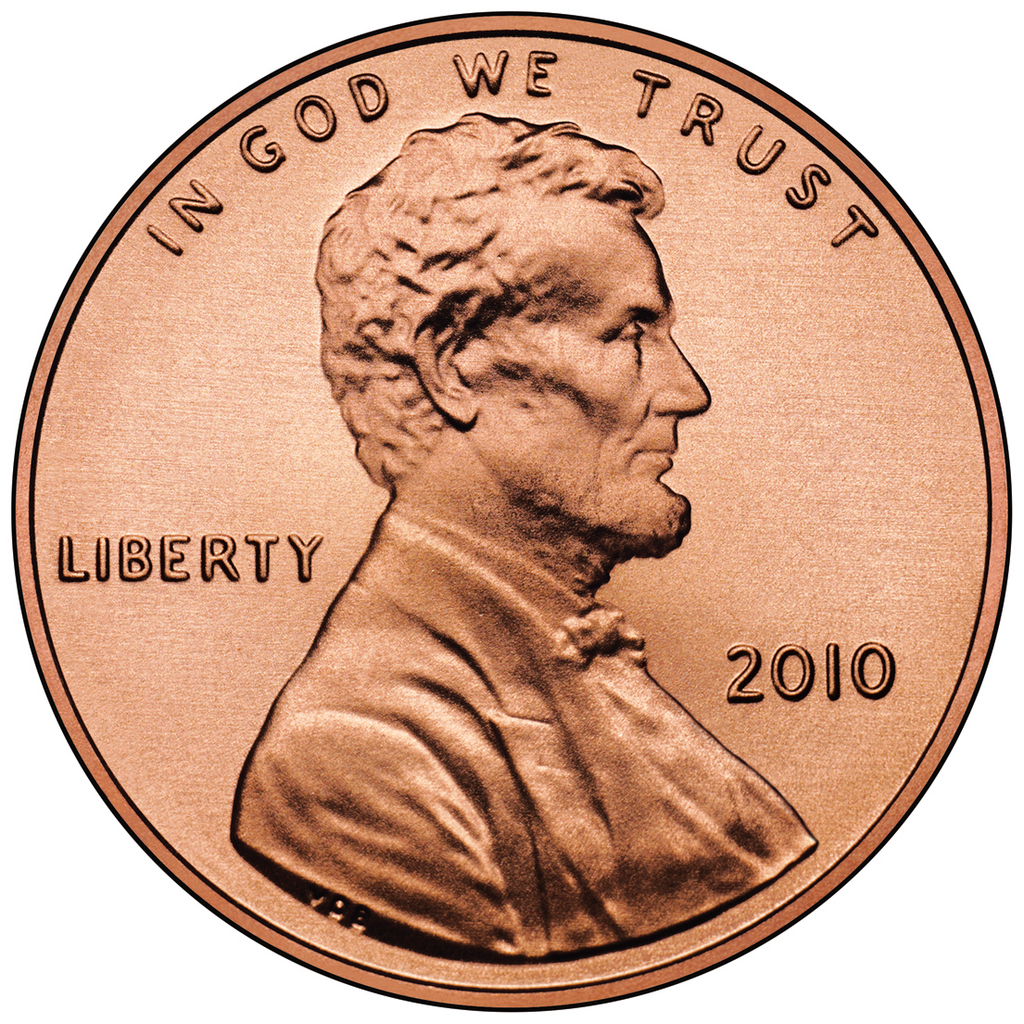
\includegraphics[scale=0.5]{coin}}
      {Image put in the public domain by the U.S. Mint.}
\end{verbatim}
produces:
\begin{center}
	\copyrightbox
		{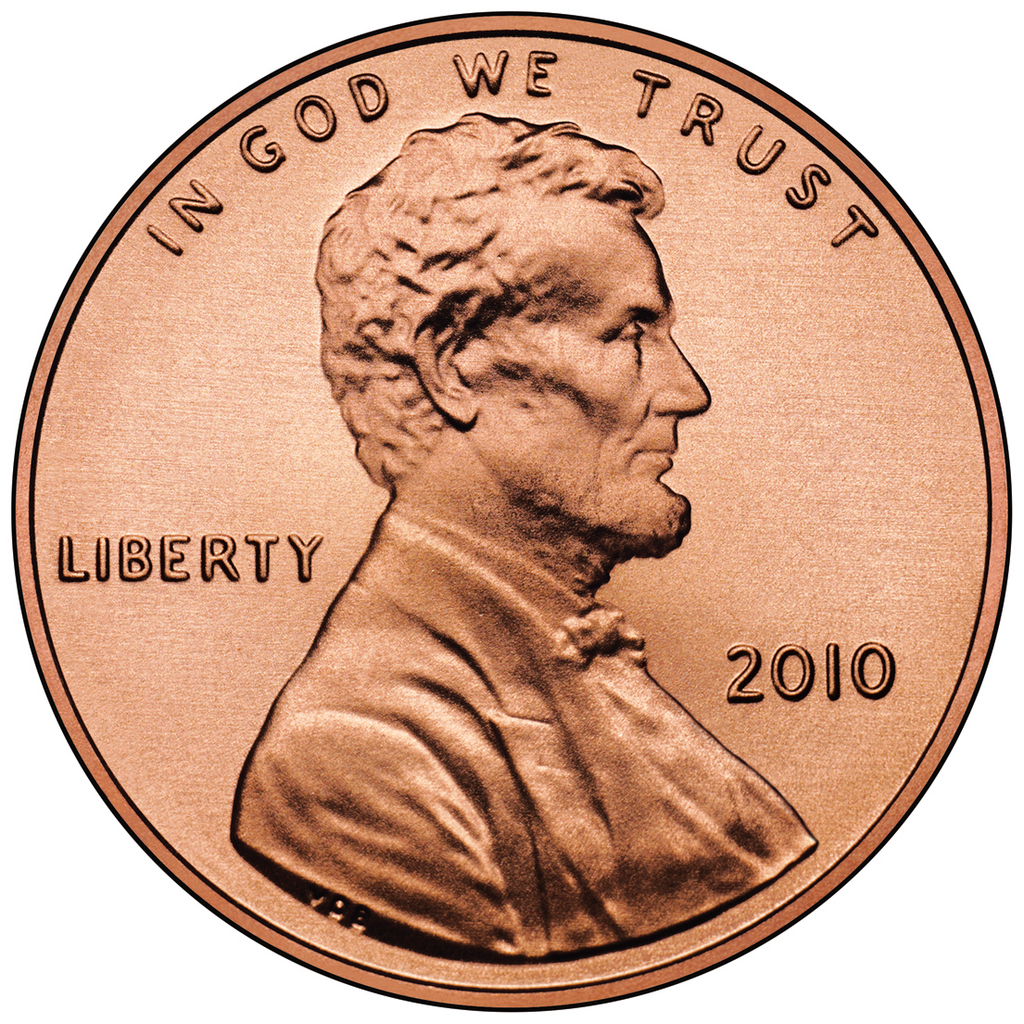
\includegraphics[scale=0.5]{coin}}
		{Image put in the public domain by the U.S. Mint.}
\end{center}

\subsection{Example 2}
The command

\begin{verbatim}
 \copyrightbox[b]
      {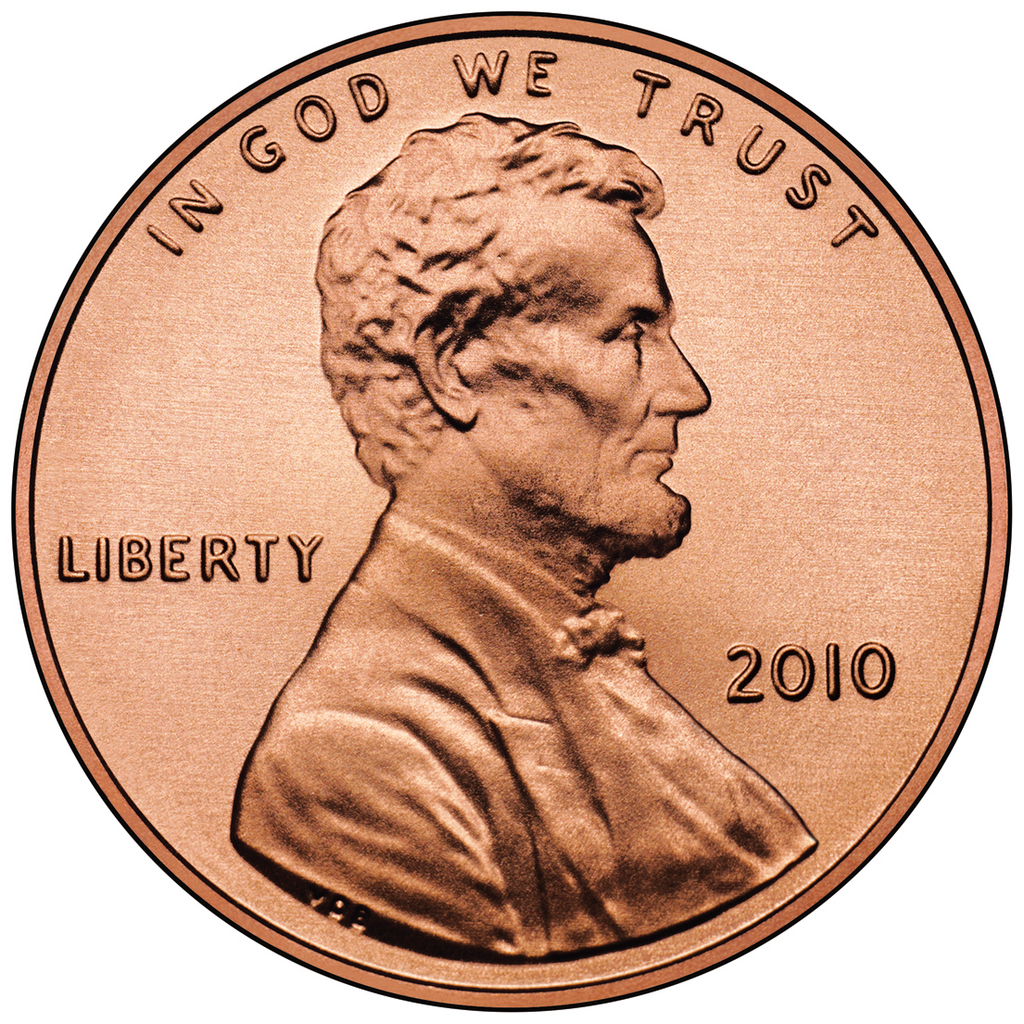
\includegraphics[scale=0.5]{coin}}
      {Image put in the public domain by the U.S. Mint.}
\end{verbatim}
produces:
\begin{center}
	\copyrightbox[b]
		{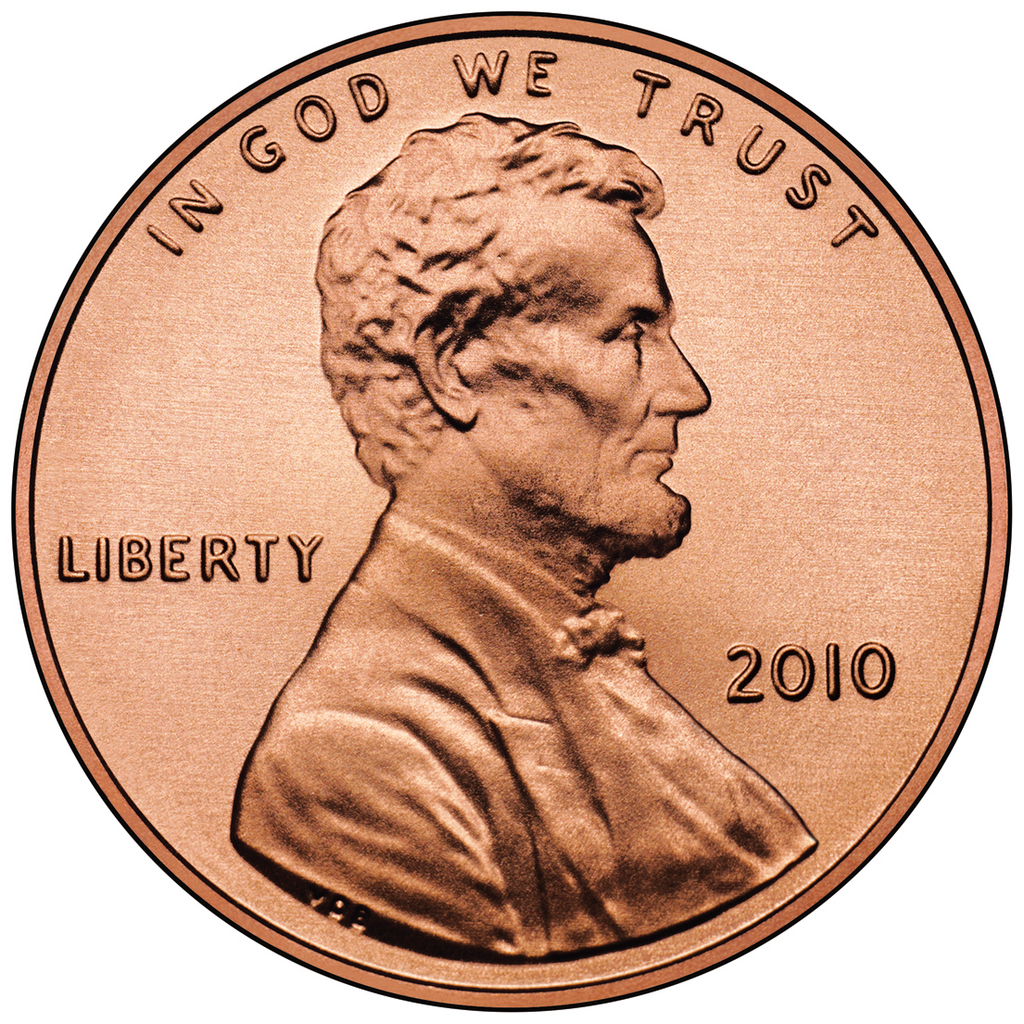
\includegraphics[scale=0.5]{coin}}
		{Image put in the public domain by the U.S. Mint.}
\end{center}


\subsection{Example 3}
The command

\begin{verbatim}
 \copyrightbox[l]
      {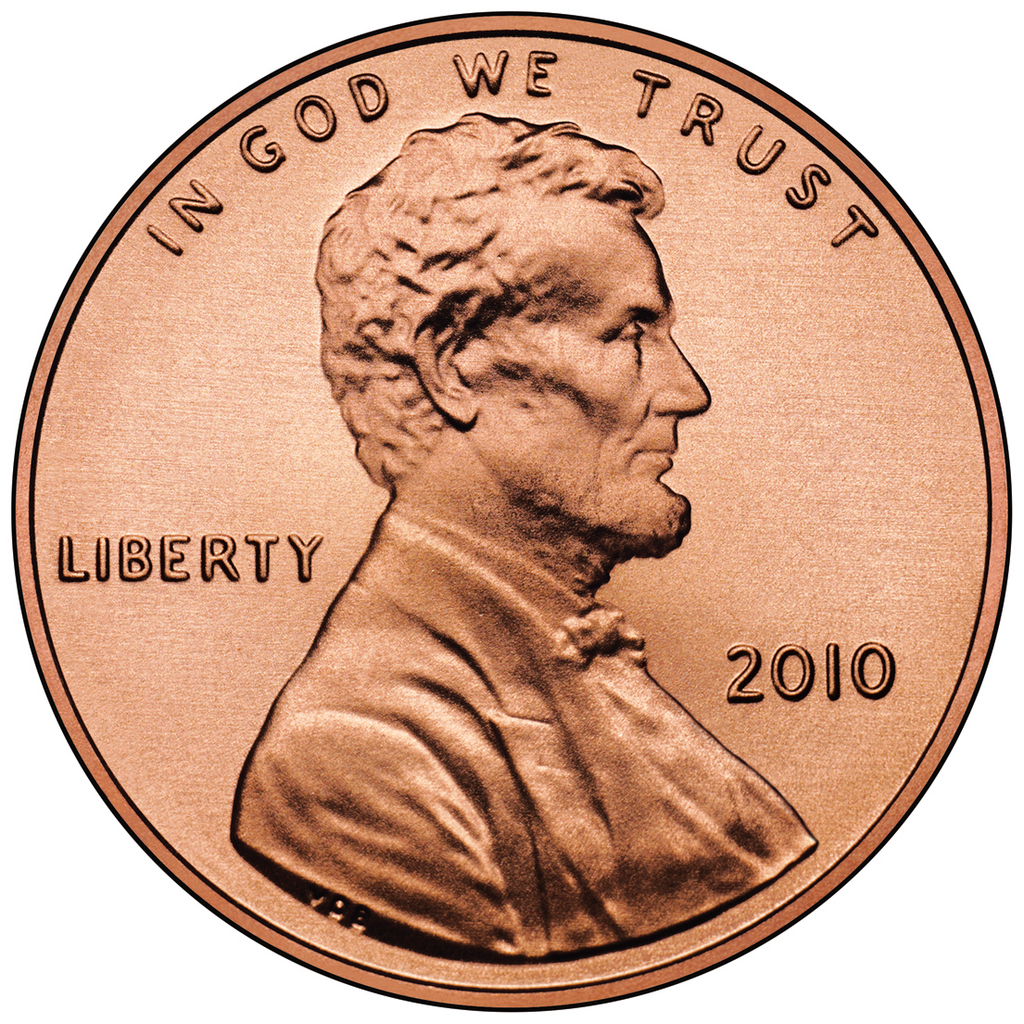
\includegraphics[scale=0.5]{coin}}
      {Image put in the public domain by the U.S. Mint.}
\end{verbatim}
produces:
\begin{center}
	\copyrightbox[l]
		{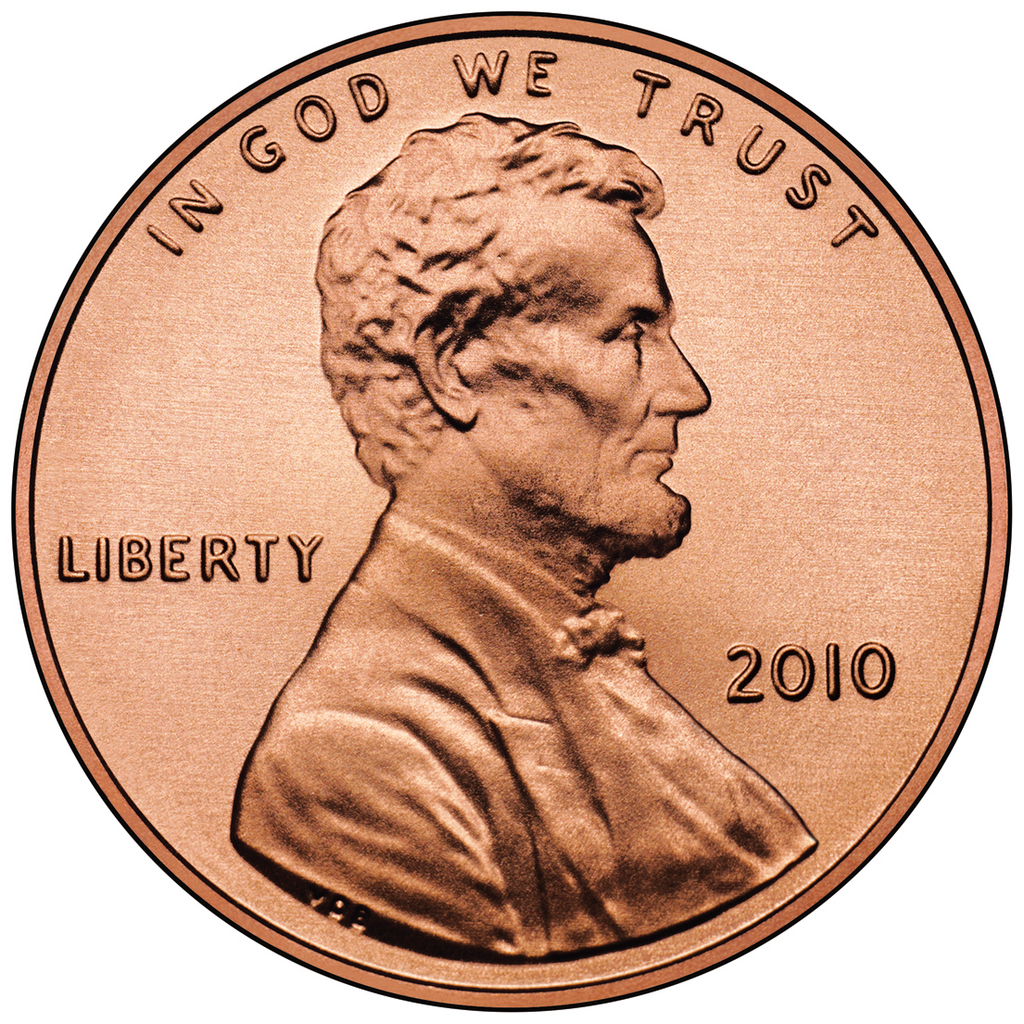
\includegraphics[scale=0.5]{coin}}
		{Image put in the public domain by the U.S. Mint.}
\end{center}


\subsection{Example 4}
\cmd{\copyrightbox} does not require \cmd{\includegraphics} images, you can
just as easily generate your own images with something like \pkg{TikZ} or the
\LaTeX\ \env{picture} environment.

For example, the command

\begin{verbatim}
\copyrightbox[r] { \tikz \filldraw[fill=green] (0,0) circle (2); }
{Image created by the author.}
\end{verbatim}
produces:
\begin{center}
\copyrightbox[r] { \tikz \filldraw[fill=green] (0,0) circle (2); }
{Image created by the author.}
\end{center}

\section{Notes}
\subsection{Changing the Font}
It's possible to change every aspect of the font used in the copyright message
by renewing the command \cmd{\CRB$@$setcopyrightfont}, for example: 

\begin{verbatim}
\makeatletter
\renewcommand{\CRB@setcopyrightfont}{%
	\footnotesize 
	\color{red!33}
	\sc
}
\makeatother

\copyrightbox[r] { \tikz \filldraw[fill=green] (0,0) circle (2); }
{Image created by the author.}
\end{verbatim}
can be placed anywhere in your .tex file and will generate the copyright notice in small caps in a reddish tint:
\begin{center}
\makeatletter
\renewcommand{\CRB@setcopyrightfont}{%
	\footnotesize 
	\color{red!33}
	\sc
}
\makeatother

\copyrightbox[r] { \tikz \filldraw[fill=green] (0,0) circle (2); }
{Image created by the author.}
\end{center}

\subsection{Justification}
Although it's not exactly recommended, it is possible to place relatively
large amounts of text near images. Long amounts of text are usually nicer to
look at when justified, and to do so \cmd{\renewcommand}
\cmd{\CRB@setcopyrightparagraphstyle} to something other than
\cmd{\raggedright}, which is the default. 

Place

\begin{verbatim}
\makeatletter
\renewcommand{\CRB@setcopyrightparagraphstyle}{%
% Return to justifying text
\setlength{\rightskip}{0pt}
\setlength{\leftskip}{0pt}
}

\makeatother
\begin{center}
	\copyrightbox[r]
		{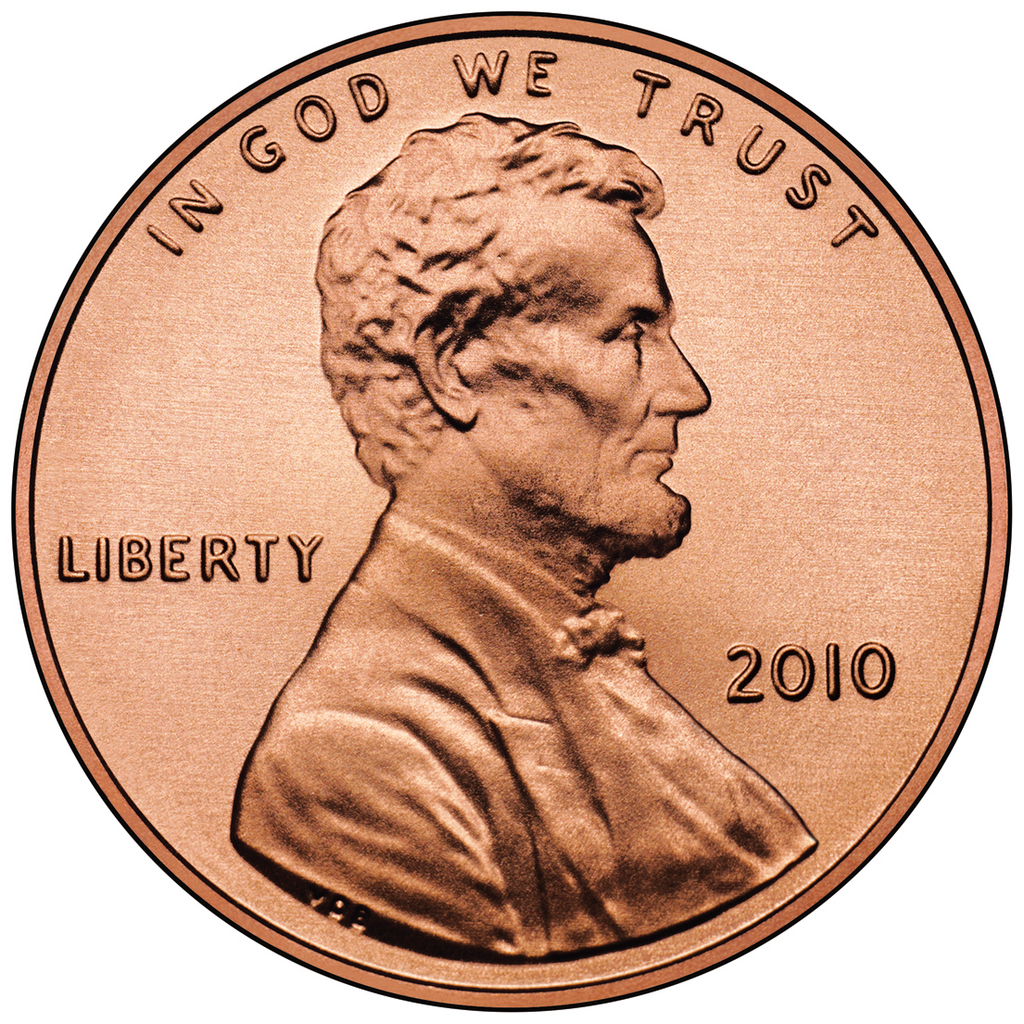
\includegraphics[scale=0.5]{coin}}
      {This here image was put in the public domain some time ago by the U.S. Mint.}
\end{center}
\end{verbatim}

anywhere in your .tex file to produce:
\makeatletter
\renewcommand{\CRB@setcopyrightparagraphstyle}{%
% Return to justifying text
\setlength{\rightskip}{0pt}
\setlength{\leftskip}{0pt}
}

\makeatother
\begin{center}
	\copyrightbox[r]
		{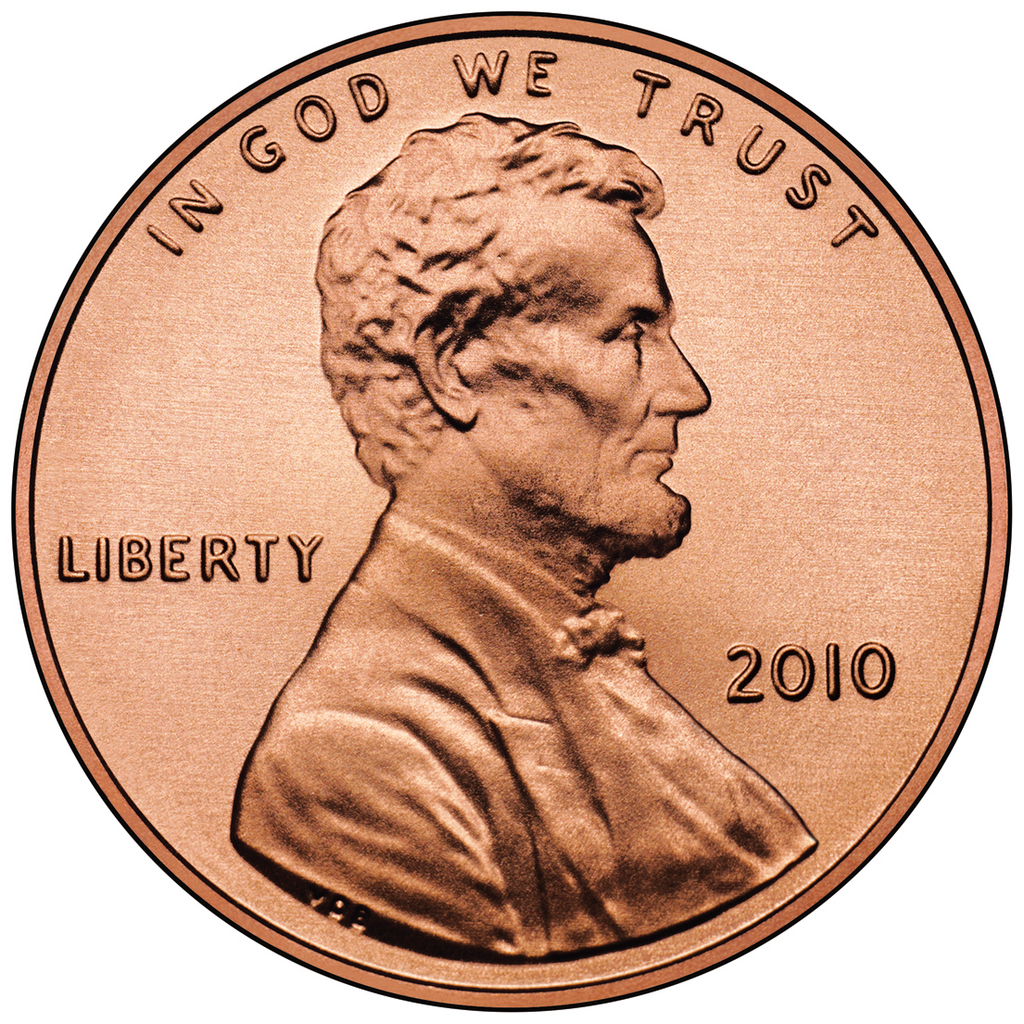
\includegraphics[scale=0.5]{coin}}
      {This here image was put in the public domain some time ago by the U.S. Mint.}
\end{center}

instead of 

\makeatletter
\renewcommand{\CRB@setcopyrightparagraphstyle}{%
% Return to justifying text
\raggedright
}

\makeatother
\begin{center}
	\copyrightbox[r]
		{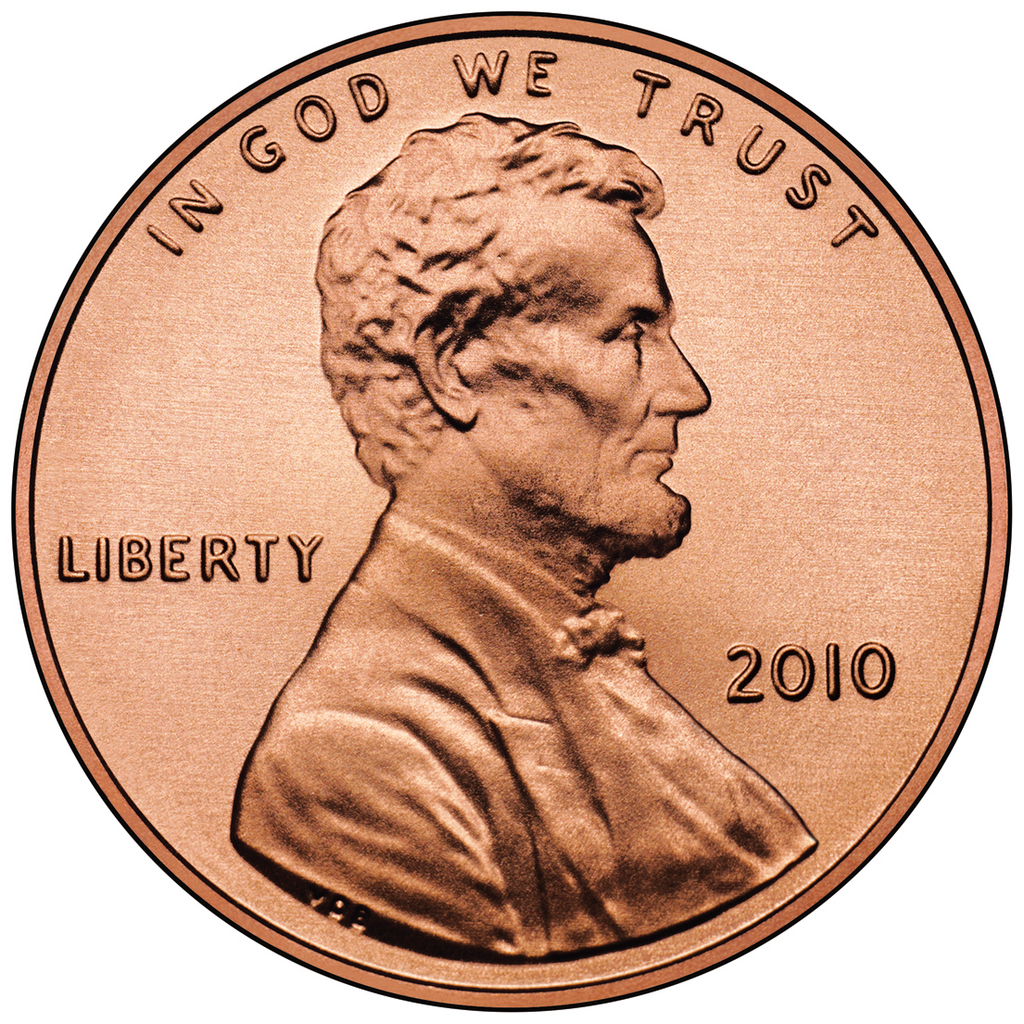
\includegraphics[scale=0.5]{coin}}
      {This here image was put in the public domain some time ago by the U.S. Mint.}
\end{center}

\section{Bugs and Suggestions}
Bugreports, suggestions and patches are welcome and can be emailed to
\mail{ives.vdf@gmail.com}, or you can fork
\url{https://github.com/Ivesvdf/copyrightbox} and send me a pull request
through Github. 
\end{document}
